\chapter{Reinterpretation}
\label{chap:reinterpretation}

In Section ~\ref{sec:results}, we presented our observed yields in the signal region and found they were consistent with the background expectations. We chose to apply these results


In light of this, we set upper limits esented in the context of setting lower limits on the mass of gluinos in a supersymmetric model. 

mass for specific the T5HH and T5ZH models. Many such SMS models exist within the MSSM which predict the production of high-$p_{T}$ bosons and it is therefore important to include information necessary to make predictions of yields for different final states. This is aided by providing the interested party with efficiencies for $b\bar{b}$ tagging and mass tagging of the AK8 jets. Tagging efficiencies for the five largest decay modes relevant to the analysis for the H boson are seen in \ref{fig:effH}. Tagging efficiencies for the hadronic decay modes of the Z boson are seen in Figure~\ref{fig:effZ}, the much lower mass tagging efficiency for the Z boson is due to our choice of signal mass window [85, 135 GeV] not being optimal for Z boson reconstruction. These are used to calculate the expected yields in the 6 analysis regions when performing a reinterpretation of the analysis using different final states. 

For each event, the yield in each bin can be predicted by first forming the following weights using the tagging efficiencies for the two highest p$_{T}$ AK8 jets as seen below. j0 and j1 represent the highest and second highest p$_{T}$ AK8 jet, respectively. The weights on the right-hand-side are $p_{T}$ dependent.

\begin{itemize}
\item double mass tag weight = $j0_{signalmass} \cdot j1_{signalmass}$
\item anti mass tag weight = $(j0_{sidebandmass} \cdot j1_{signalmass}) + (j1_{signalmass} \cdot j1_{sidebandmass}) + (j0_{sidebandmass} \cdot j1_{sidebandmass})$
\item double bb tag weight = $j0_{bbtag} \cdot j1_{bbtag}$
\item single bb tag weight = $(j0_{bbtag} \cdot (1-j1_{bbtag})) + ((1-j0_{bbtag})\cdot j1_{bbtag})$
\item anti bb tag weight = $(1-j0_{bbtag}) \cdot (1-j1_{bbtag}$)
\end{itemize}

These weights are then combined in the following manner to determine the yields across each of the 6 bins for a single event.

\begin{enumerate}
\item A1 weight = (single bb tag weight) $\cdot$ (double mass tag weight)
\item A2 weight = (double bb tag weight) s$\cdot$ (double mass tag weight)
\item B1 weight = (single bb tag weight) $\cdot$ (anti mass tag weight)
\item B2 weight = (double bb tag weight) $\cdot$ (anti mass tag weight)
\item C weight = (anti bb tag weight) $\cdot$ (double mass tag weight)
\item D weight = (anti bb tag weight) $\cdot$ (anti mass tag weight)
\end{enumerate}

These weights for the 6 analysis bins (inclusive in \ptmiss) are then summed over all events to get the expected yields.
The prescription was tested using the T5HH model with a gluino mass of 2200 GeV and compared it to the true value.
The largest deficit was in the D region, with a difference of -36\% difference from nominal.
The greatest over-prediction is found in the B2 region, with a surplus of +8.2\% events relative to nominal.
The closure in the other bins fall somewhere in this range.
These results are summarized in Table~\ref{tab:predclos}.
As a further cross-check to the yield estimates, Table~\ref{tab:sigeff} shows the true signal event efficiencies for the T5HH model with a gluino mass of 2200 GeV.

\begin{figure}[hbp!]
\centering
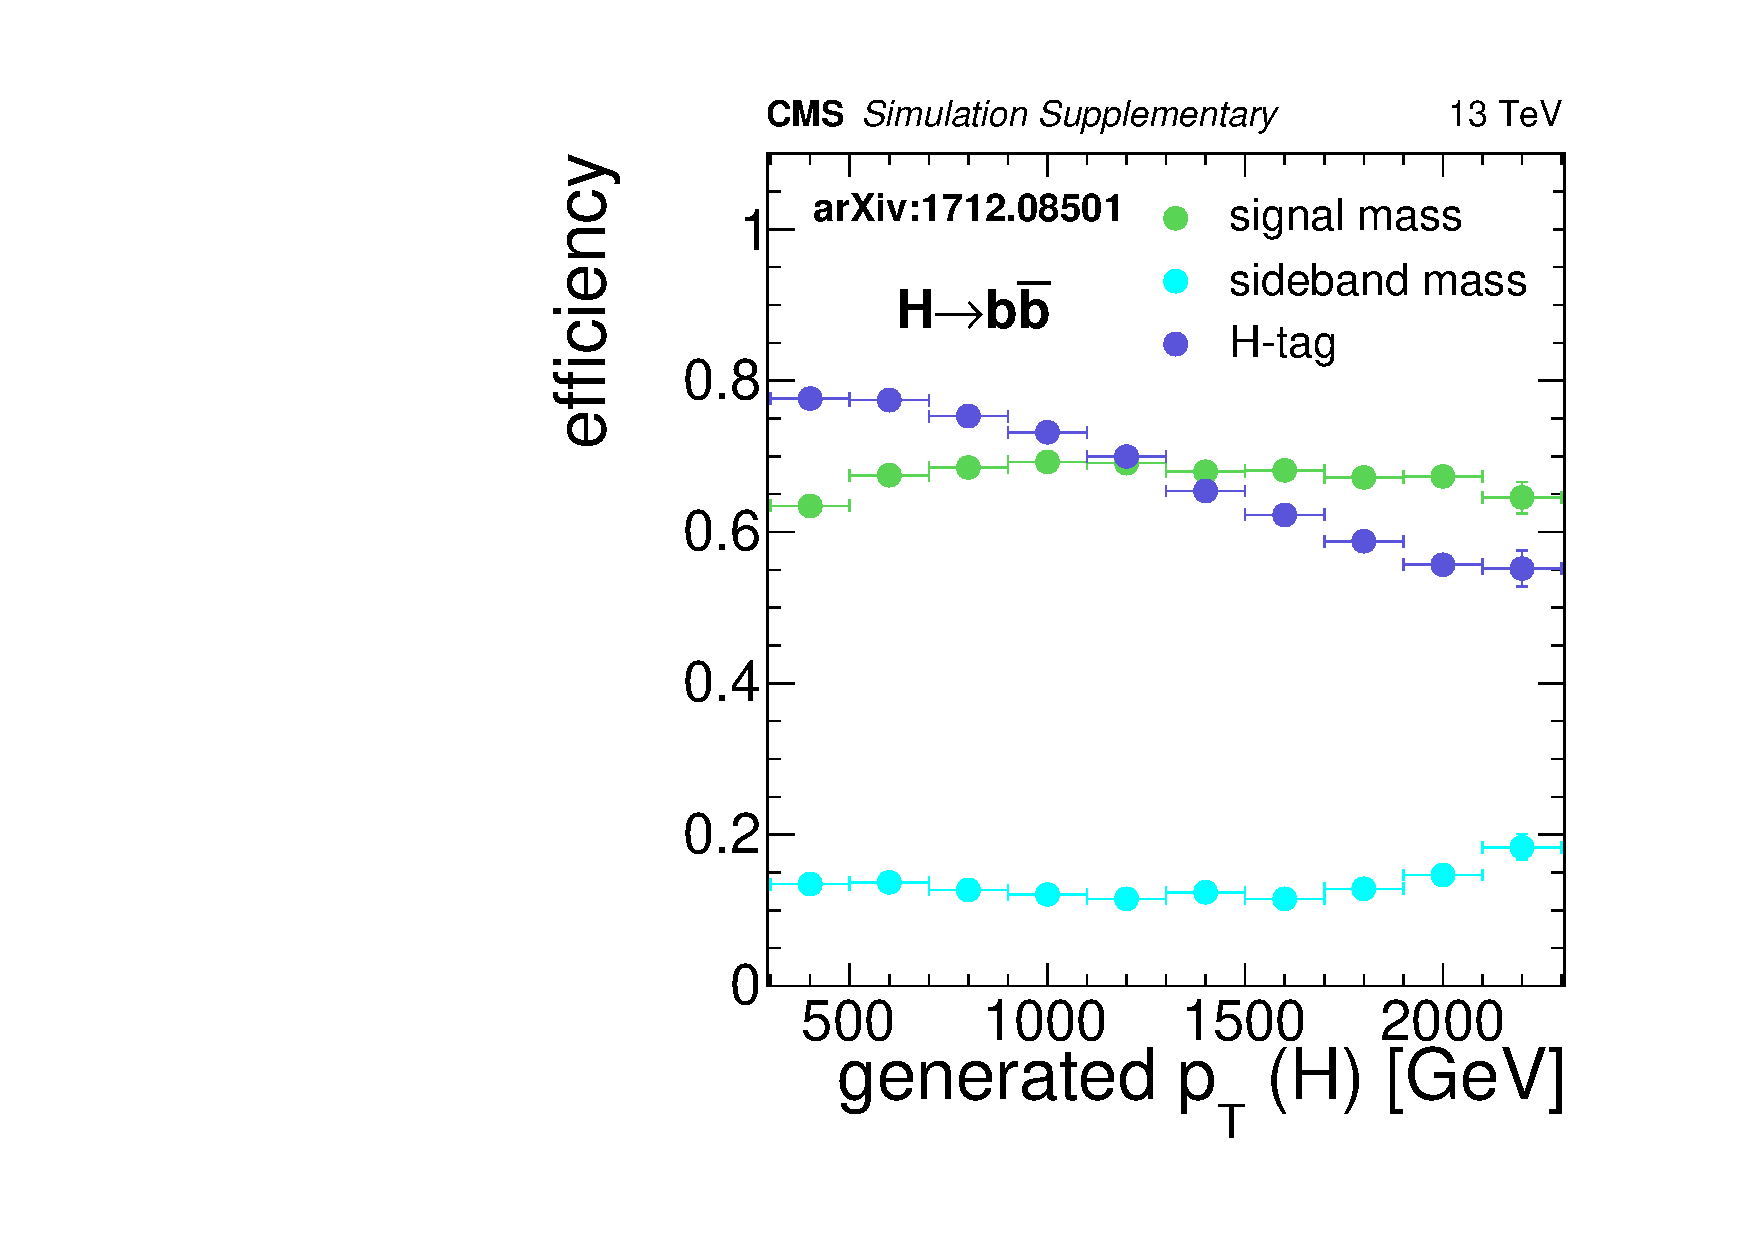
\includegraphics[width=0.425\linewidth]{figs/CMS-SUS-17-006_Figure-aux_006.pdf}
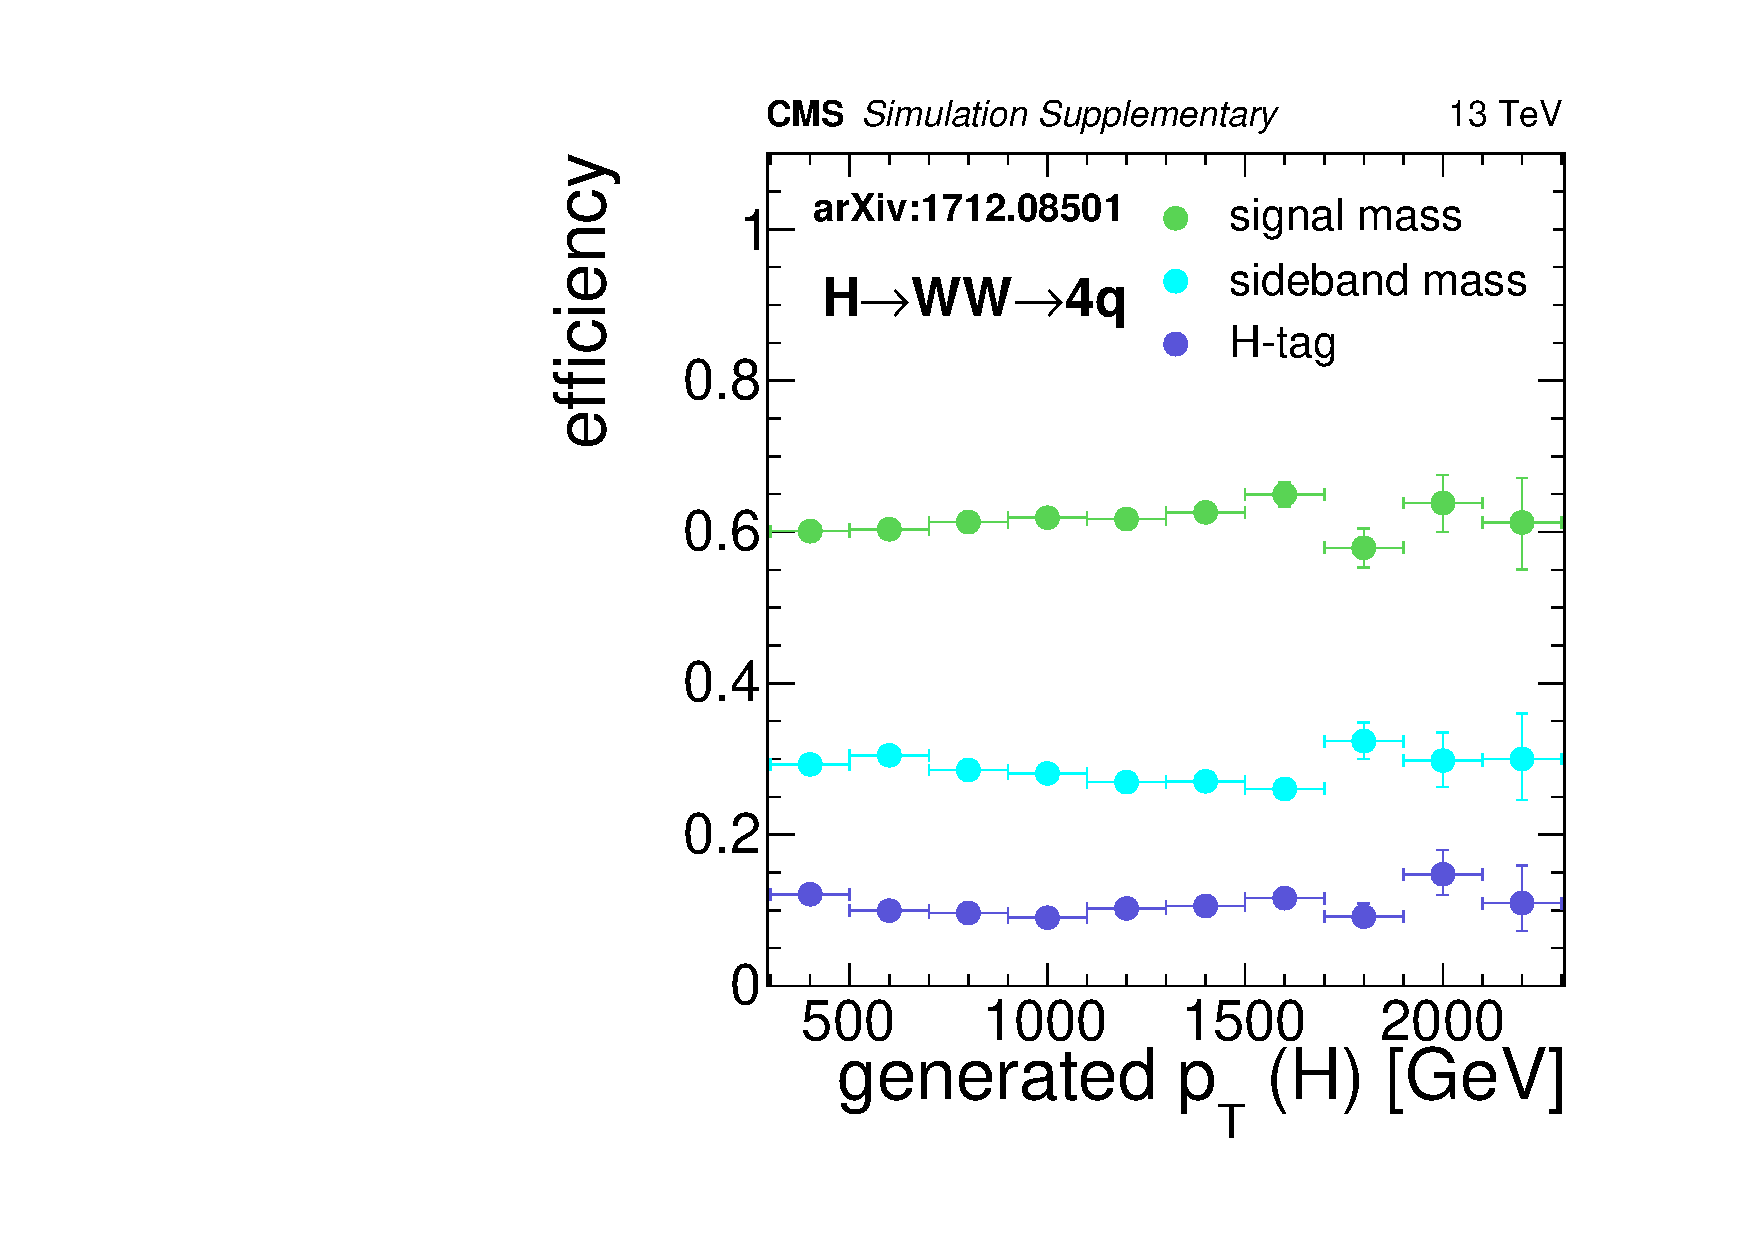
\includegraphics[width=0.425\linewidth]{figs/CMS-SUS-17-006_Figure-aux_007.pdf}
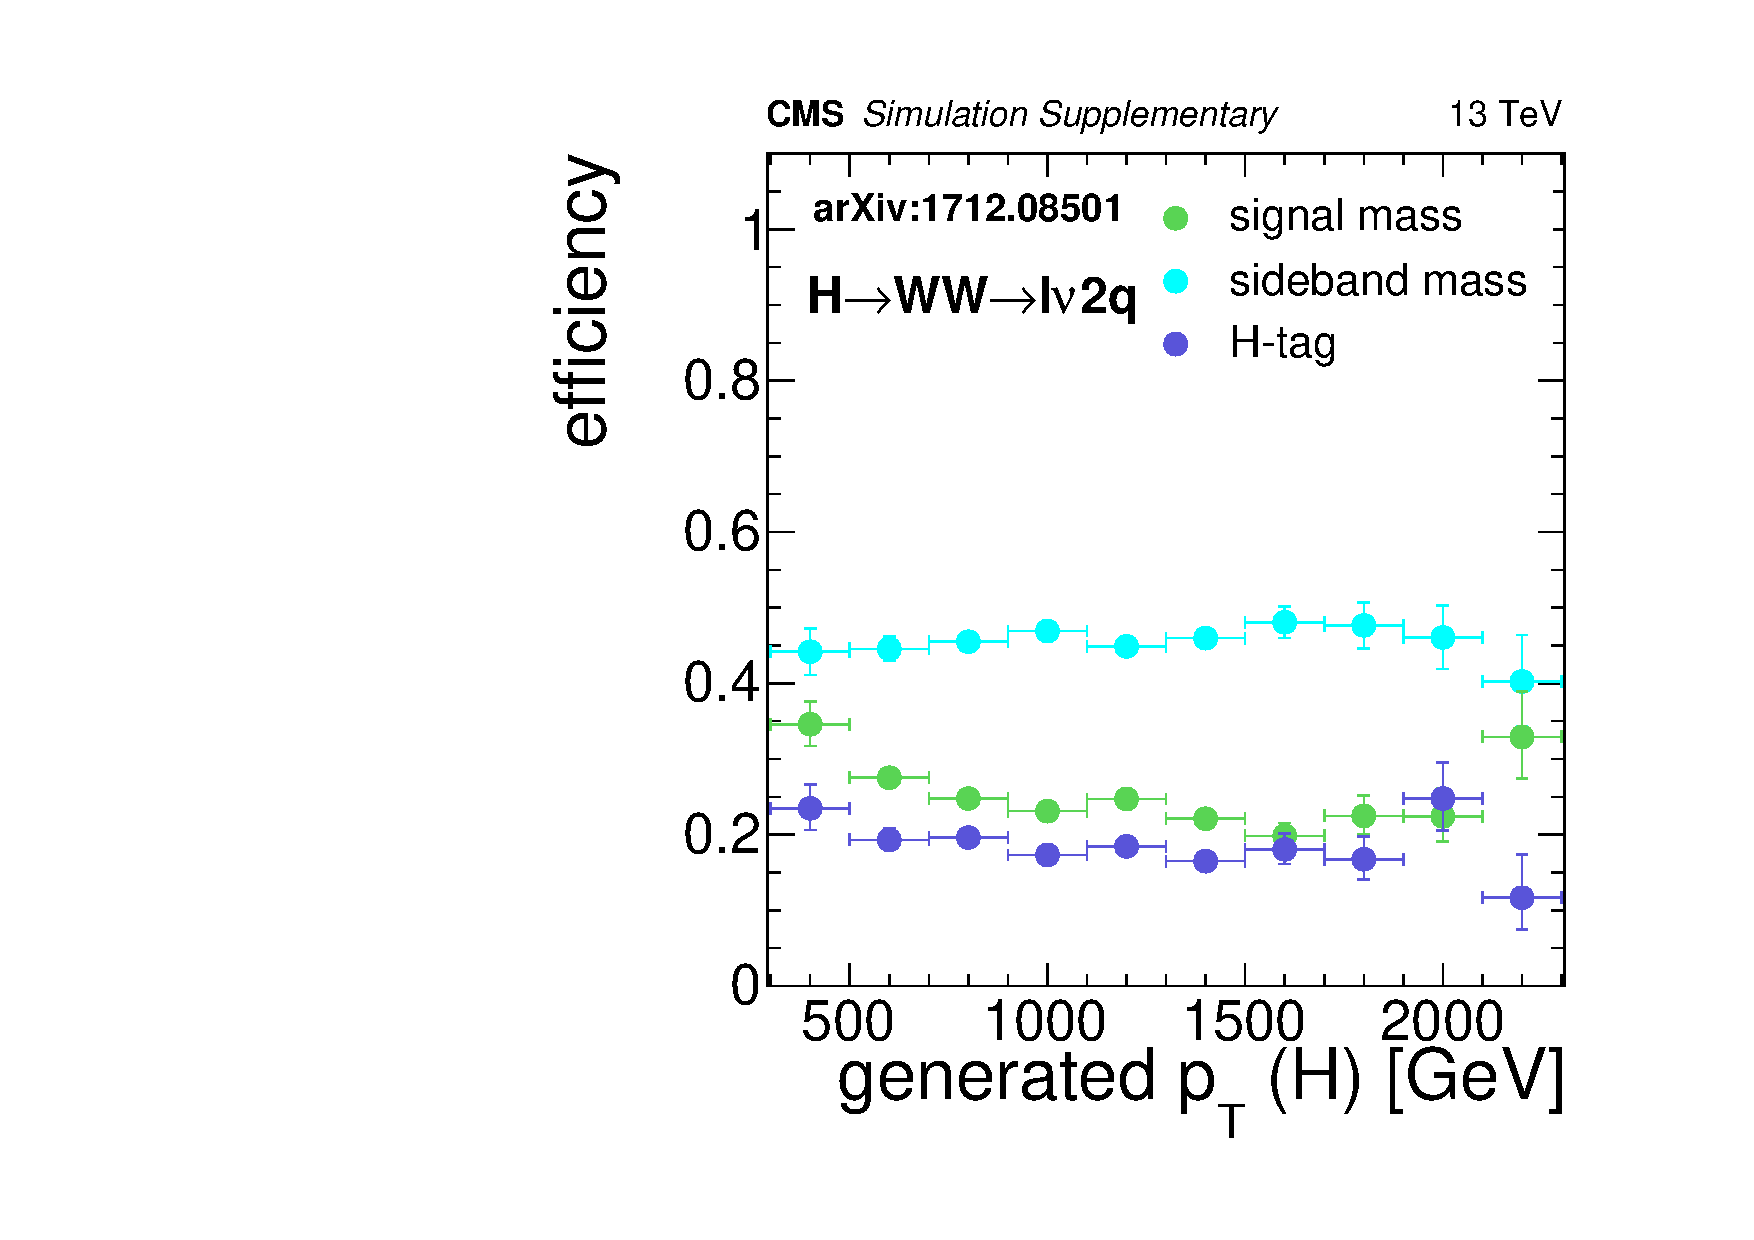
\includegraphics[width=0.425\linewidth]{figs/CMS-SUS-17-006_Figure-aux_008.pdf}
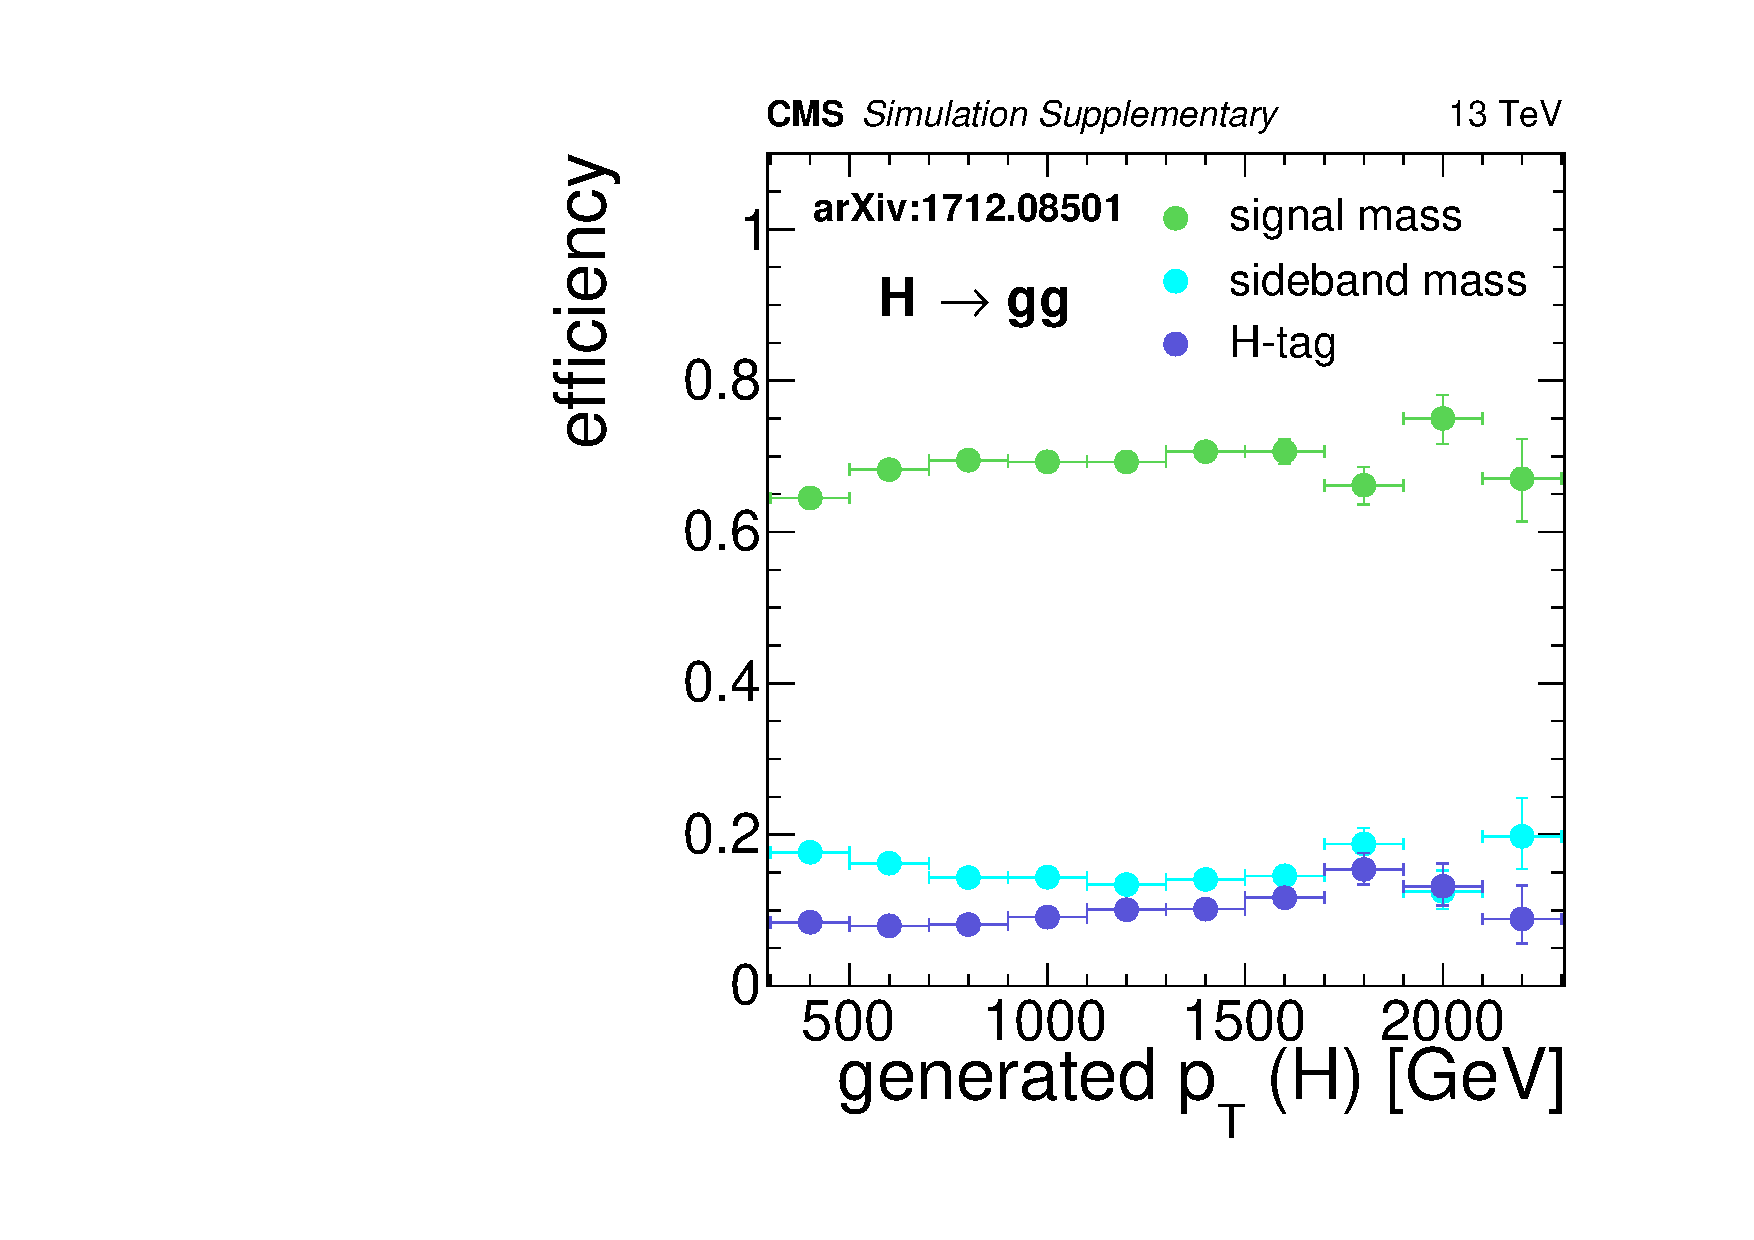
\includegraphics[width=0.425\linewidth]{figs/CMS-SUS-17-006_Figure-aux_009.pdf}
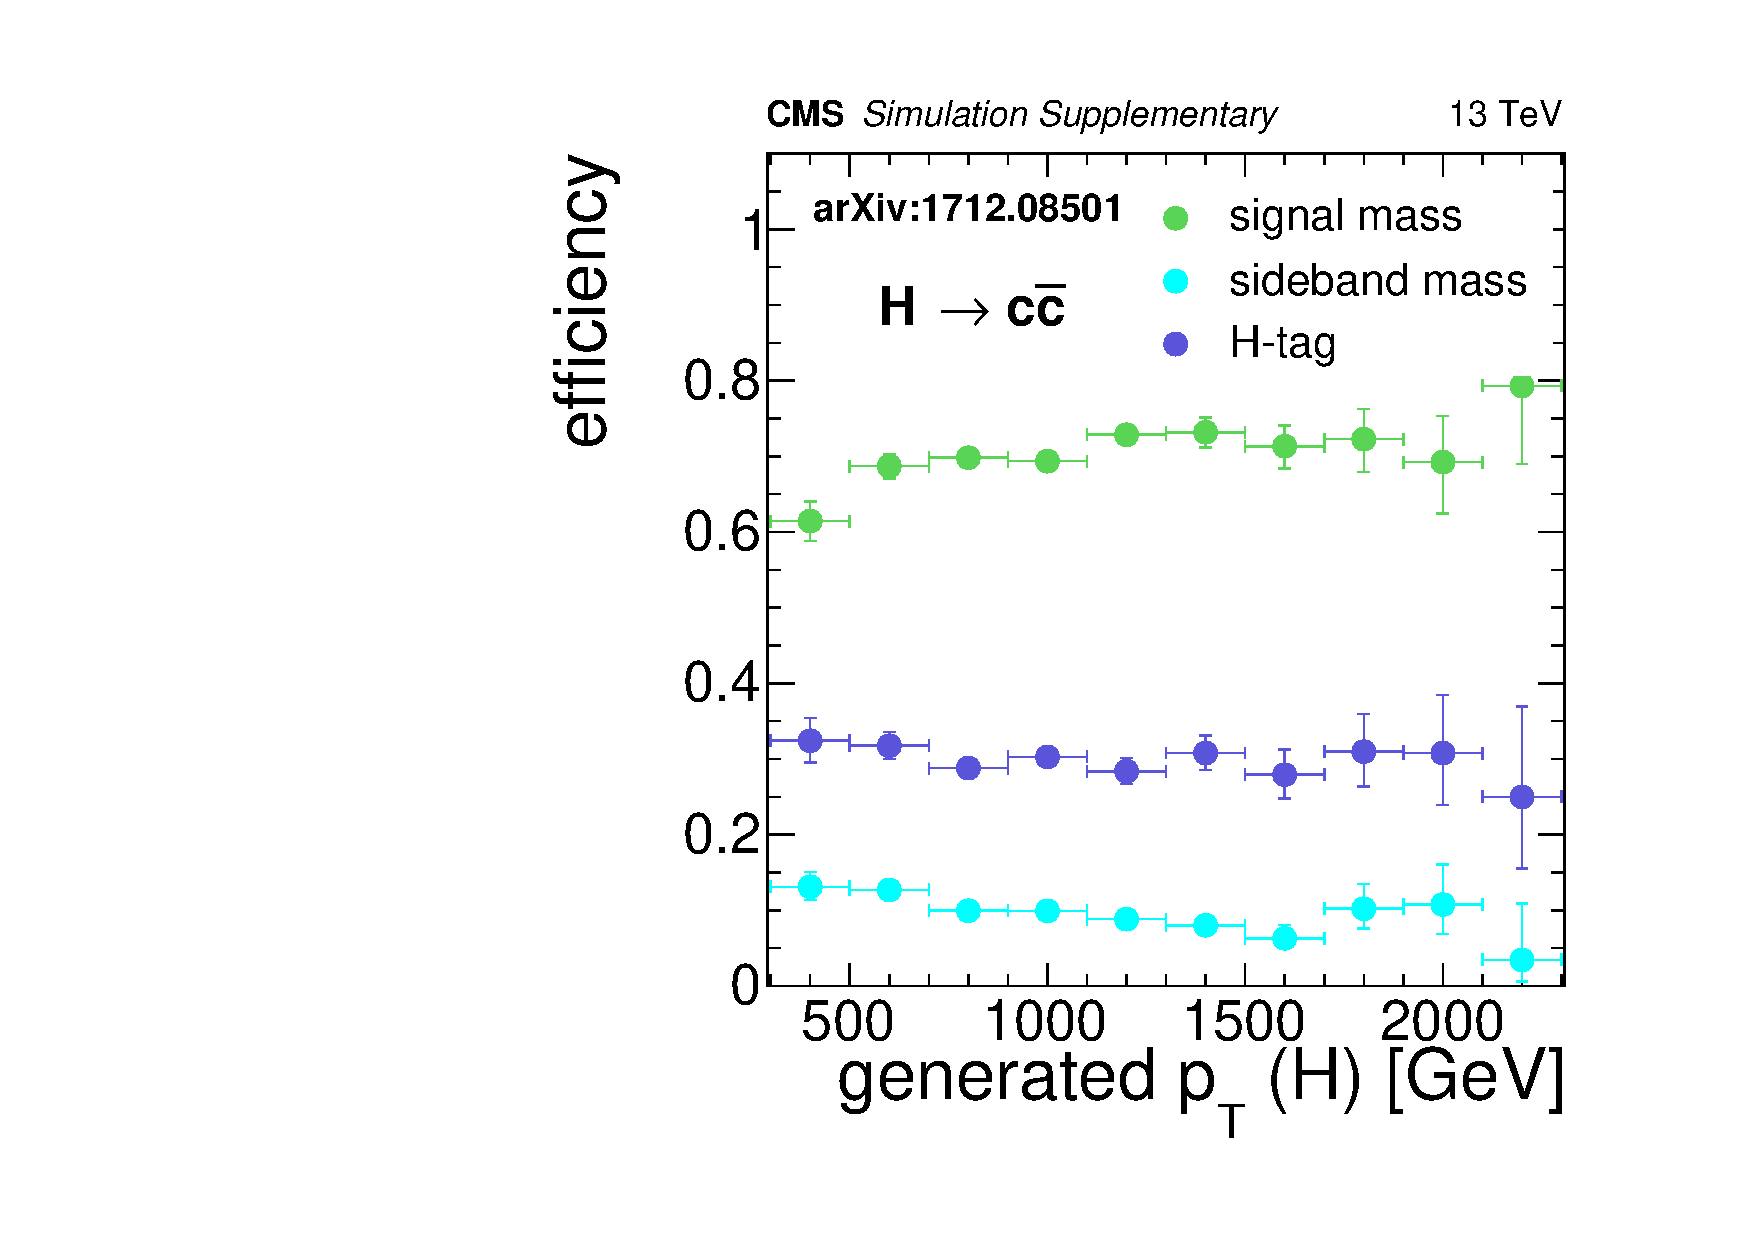
\includegraphics[width=0.425\linewidth]{figs/CMS-SUS-17-006_Figure-aux_010.pdf}

\includegraphics[width=0.425\linewidth]{figs/blankcanvas.pdf}
\caption[Efficiencies for an AK8 jet originating from H boson decay, relative to baseline selection.]{
Efficiencies for an AK8 jet originating from H boson decay, relative to baseline selection.
"signal mass" represents the probability the jet will have mass [85, 135 GeV].
"sideband mass" represents the probability the jet will have mass [50, 85 GeV] or [135, 250 GeV].
"H-tag" represents the probability the jet have a double-b discriminator value greater than 0.3, for jets with mass [50, 250 GeV].
Efficiencies were derived using the T5ZH  with a gluino mass of 2200 GeV.
}
\label{fig:effH}
\end{figure}

\begin{figure}[hbp!]
\centering
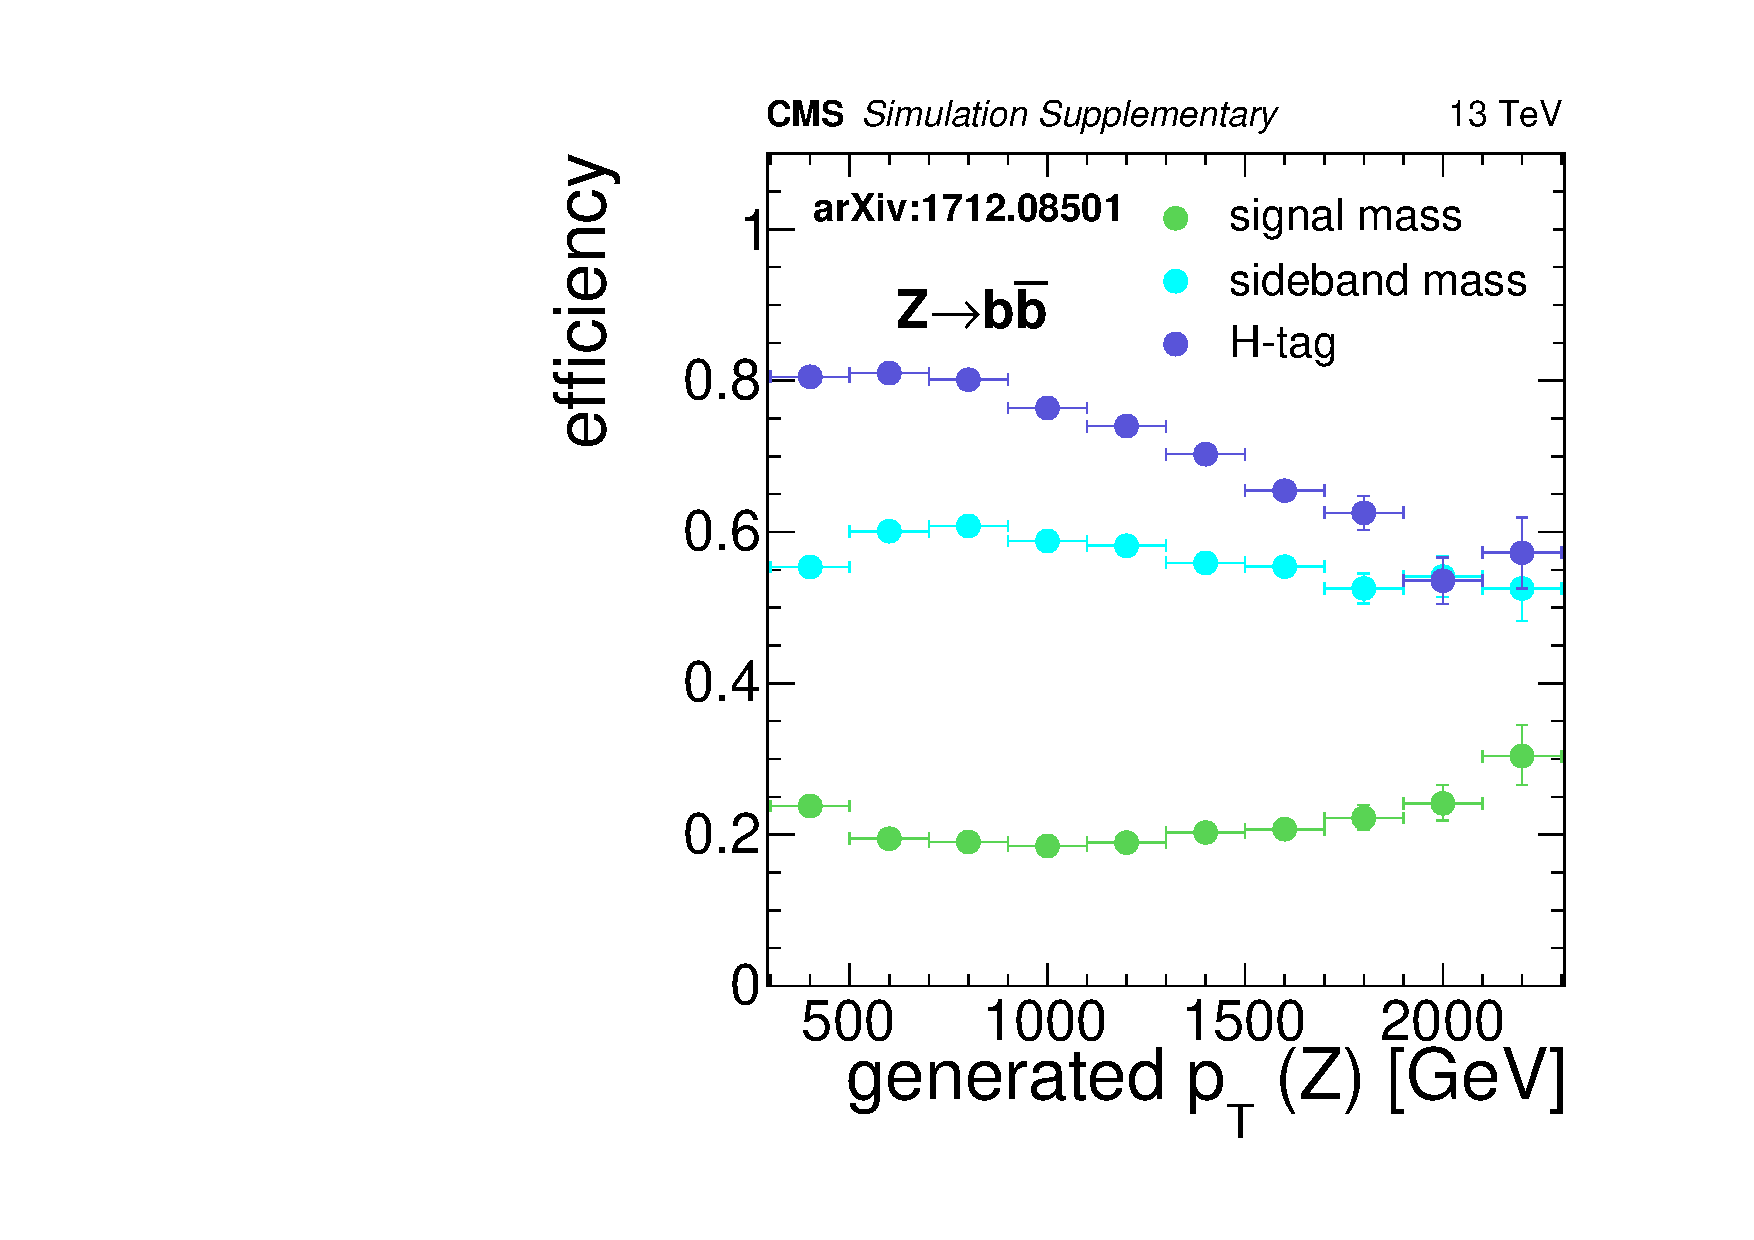
\includegraphics[width=0.425\linewidth]{figs/CMS-SUS-17-006_Figure-aux_011.pdf}
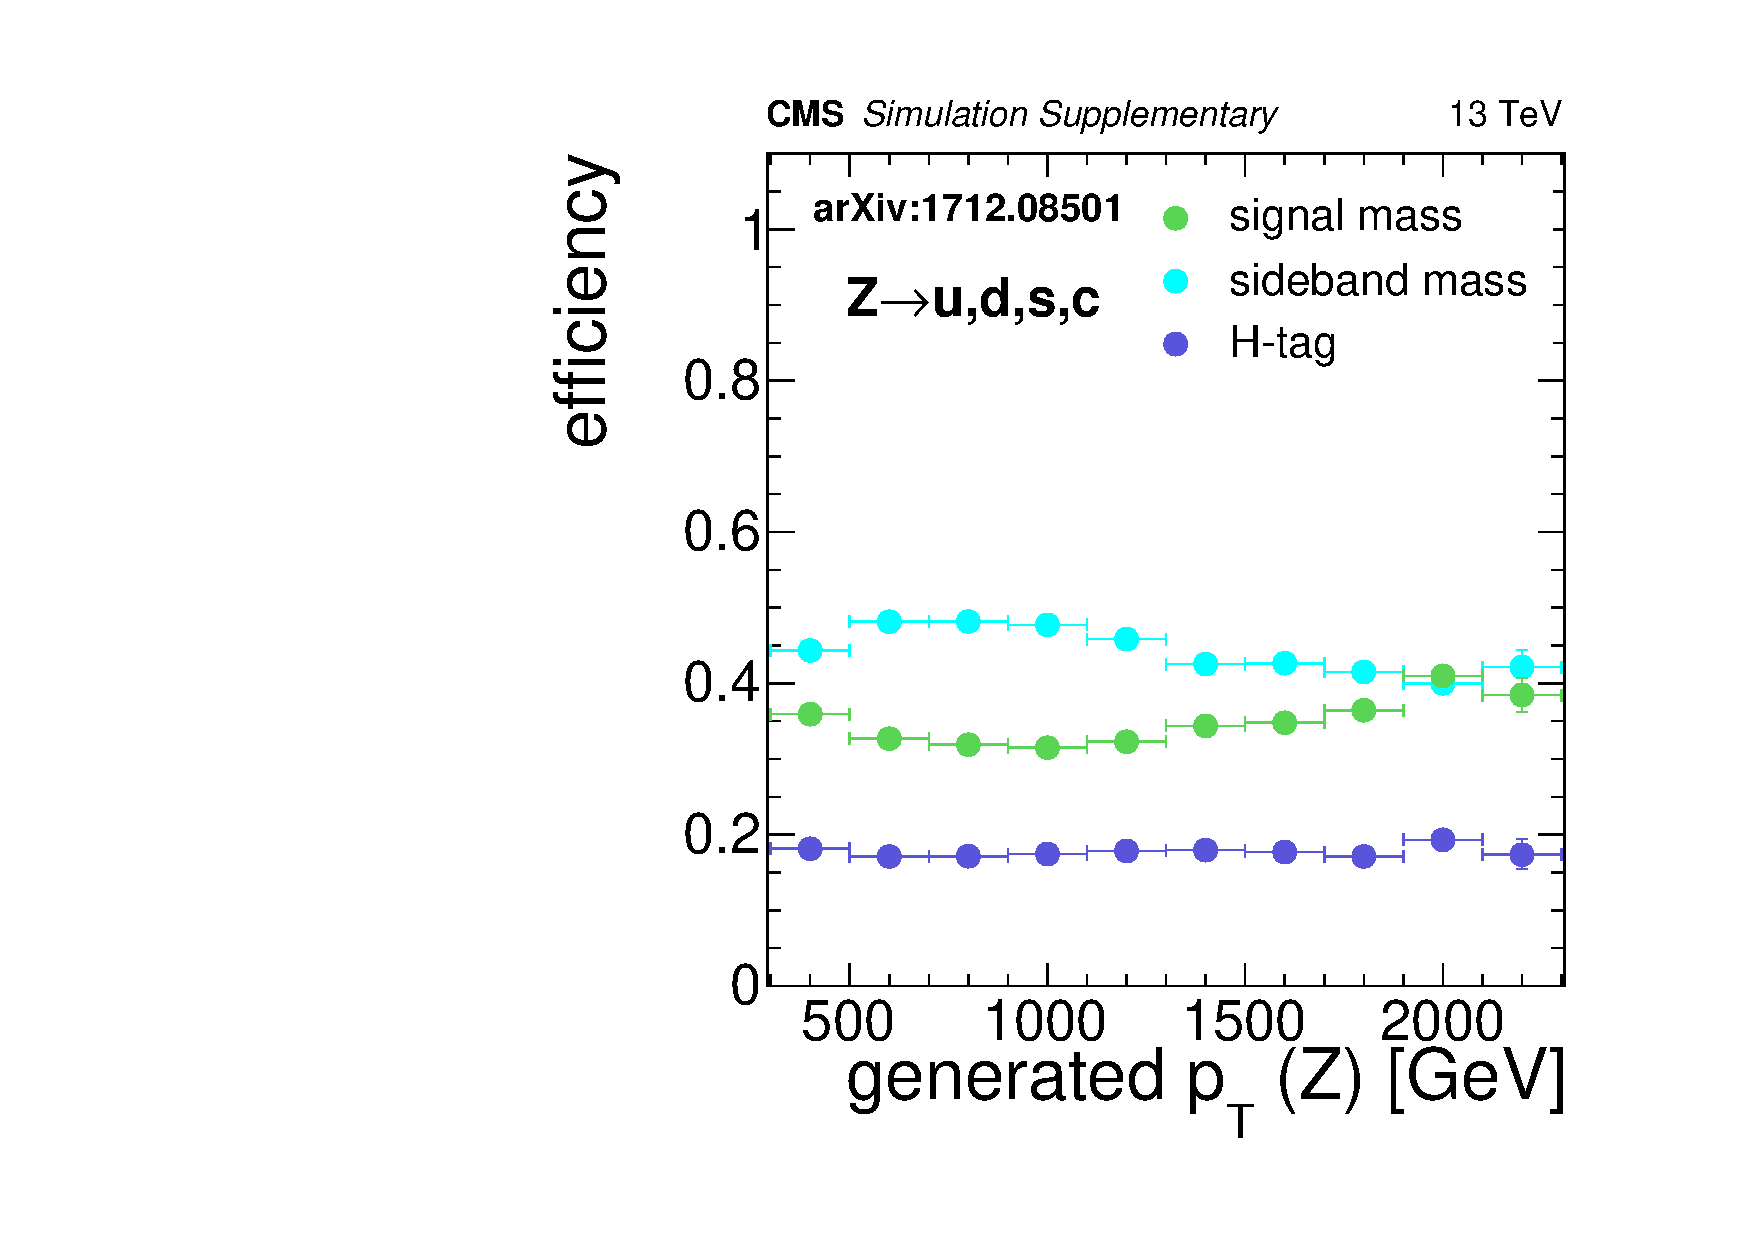
\includegraphics[width=0.425\linewidth]{figs/CMS-SUS-17-006_Figure-aux_012.pdf}
\caption[Efficiencies for an AK8 jet originating from Z boson decay, relative to baseline selection.]{
Efficiencies for an AK8 jet originating from Z boson decay, relative to baseline selection.
"signal mass" represents the probability the jet will have mass  [85, 135 GeV].
"sideband mass" represents the probability the jet will have mass [50, 85 GeV] or [135, 250 GeV].
"H-tag" represents the probability the jet have a double-b discriminator value greater than 0.3, for jets with mass [50, 250 GeV].
Efficiencies were derived using the T5ZH  with a gluino mass of 2200 GeV.
}
\label{fig:effZ}
\end{figure}

\begin{table}[hbp!]
\centering
\caption[Comparison of the true reco-level event yield with those obtained via the prediction.]{
Comparison of the true reco-level event yield with those obtained via the prediction. The columns with the RECO or GEN labels are the prediction using RECO or GEN event variables only, respectively. The prediction was made using the T5HH  with a gluino mass of 2200 GeV.
}
\begin{tabular}{c | c c c}
\hline\hline
         & RECO     & RECO           & GEN\\
         & "truth"  & prediction     & prediction\\
\hline
Baseline & 4.08     & 3.46 (-15\%)   & 3.53 (-16\%)\\
A1       & 1.21     & 1.18 (-2.3\%)  & 1.26 (+3.6\%)\\
A2       & 0.777    & 0.748 (-3.7\%) & 0.815 (+4.7\%)\\
B1       & 0.802    & 0.703 (-12\%)  & 0.664 (-21\%)\\
B2       & 0.322    & 0.338 (+5.0\%) & 0.350 (+8.2\%)\\
C        & 0.498    & 0.473 (-4.9\%) & 0.487 (-2.1\%)\\
D        & 0.478    & 0.353 (25\%)   & 0.308 (-36\%)\\
\hline\hline
\end{tabular}
\label{tab:predclos}
\end{table}

\begin{table}[hbp!]
\centering
\caption[T5HH signal event efficiencies.]{
Signal efficiencies for an event to land in a given analysis bin.
The efficiencies were derived using the T5HH  with a gluino mass of 2200 GeV.
Choosing a gluino mass of 1800 GeV decreases the efficiencies by a relative 5\%.
}
\begin{tabular}{c | c c c c c c c c}
\hline
\hline
                                                            & Baseline & A1     & A2      & B1      & B2      & C       & D\\
\hline
$p_{\mathrm{T}}^{\mathrm{miss}}< 300\,\mathrm{GeV}$        & 32\%    & 9.4\%   & 6.0\%   & 6.2\%   & 2.5\%   & 3.9\%   & 3.7\% \\
$300 < p_{\mathrm{T}}^{\mathrm{miss}} < 500\,\mathrm{GeV}$  & 2.7\%   & 0.78\%  & 0.52\%  & 0.54\%  & 0.25\%  & 0.31\%  & 0.30\% \\
$500 < p_{\mathrm{T}}^{\mathrm{miss}} < 700\,\mathrm{GeV}$  & 3.5\%   & 1.0\%   & 0.65\%  & 0.72\%  & 0.28\%  & 0.43\%  & 0.40\% \\
$p_{\mathrm{T}}^{\mathrm{miss}} > 700\,\mathrm{GeV}$        & 26\%    & 7.6\%   & 4.9\%   & 5.0\%   & 2.0\%   & 3.1\%   & 3.0\% \\
\hline
\hline
\end{tabular}
\label{tab:sigeff}
\end{table}

\begin{table}[hbp!]
\centering
\caption
[T5HH/ZH signal event cutflow.]
{T5HH and T5ZH signal efficiencies cutflow for two different gluino masses. The first row represents no selection, the final row represents the selection for the ``A$_{2}$'' signal event bin of the main analysis (inclusive in $p_{T}$).
}
\label{tab:}
\begin{tabular}{r r c c c c}
\hline
\hline
  & Model                                                                                       & HH & HH & ZH & ZH\\
  & Gluino mass (GeV)                                                               & 1300 & 2200 &1300 & 2200\\
\hline
   & Total yield at 35.9 fb$^{-1}$                        & 1660 & 12.8 & 1651 & 12.9\\
+ & Lepton \& isolated track vetoes                                              & 1253 & 10.1 & 1277 & 10.3\\
+ & $\Delta\phi_{1, 2, 3, 4}$                                                            & 1037 & 8.3 & 1049 & 8.4\\
+ & $\mathrm{HT}>600$ \& $p_{\mathrm{T}}^{\mathrm{miss}}>300$ GeV    & 886 & 7.8 & 834 & 7.6\\
+ & $\geq$2 AK8 jets with $p_{\mathrm{T}}>$ 300 GeV                     & 602 & 6.5 & 523 & 5.4\\
+ & Jet 1,2 mass $\epsilon$ [50, 250 GeV]                                  & 374  & 4.1 & 313 & 3.3\\
+ & Jet 1,2 mass $\epsilon$ [85, 135 GeV]                                  & 209  & 2.5 & 101 & 1.0\\
+ & One or two H-tags                                    & 168  & 2.0 & 67 & 0.6\\%+ & Two $b\bar{b}$-tags                                   
\hline
\hline
\end{tabular}
\end{table}
